\section{Derivation of quantum graph problem} \label{sec:ScalarDerivation}
In this section we provide an overview of a system of the form \eqref{eq:SingularWaveEqnQGProblem} is obtained from \eqref{eq:SingularScalarWaveEqn}, which will setup our discussion revolving around the methods we employ for solving \eqref{eq:SingularWaveEqnQGProblem} in section \ref{sec:ScalarDiscussion}.
However, before doing so we provide the reader with an intuitive understanding, stemming from the analysis of section \ref{sec:3DGradSobSpaces}, of the space $\tgradSob{\ddom}{\dddmes}$.
Upon deriving the quantum graph problem \eqref{eq:SingularWaveEqnQGProblem}, we will elaborate its link to our variational problem in the context of Strauss extensions, setting up our discussion in section \ref{ssec:GRandSELinks} and work in chapters \ref{ch:CurlCurl} and \ref{ch:SingInc}.

\subsection{Geometric Interpretation} \label{ssec:3DGradGeometric}
The intuition behind the form of the tangential gradients (and gradients of zero) with respect to the various measures $\lambda_{jk}, \ddmes, \nu$, and $\dddmes$ can be summarised with the colloquial phrase ``tangential gradients only reflect behaviour that the measure can see".
Let us be more precise, and first consider the measure $\lambda_{jk}$ for a fixed $I_{jk}$ and the associated gradients of zero and tangential gradients.
Suppose that we have a (sufficiently smooth) function $u$ defined on $\ddom$ that satisfies $u=0$ (or any constant value) on $I_{jk}$, from the perspective of $\lambda_{jk}$ this $u$ is the zero function,\footnote{more precisely, $u$ is represented by the zero function in $\ltwo{\ddom}{\lambda_{jk}}$.} regardless of whether $u$ is zero on the whole of $\ddom$ or not.
So despite $u=0$ in $\ltwo{\ddom}{\lambda_{jk}}$, it can have any profile in the direction $n_{jk}$ \emph{as it crosses} $I_{jk}$ and thus any kind of (reasonable) behaviour in the rest of $\ddom$ --- this is schematically illustrated in figure \ref{fig:Diagram_GradZeroIllustrations}.
\begin{figure}[b!]
	\centering
	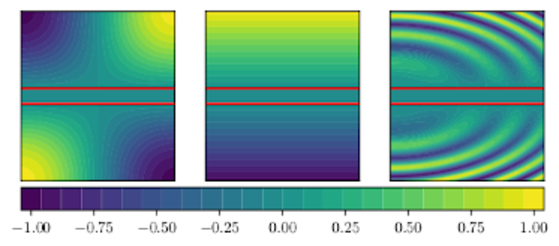
\includegraphics[scale=1.0]{Diagram_GradZeroIllustrations-Scaled.pdf}
	\caption{\label{fig:Diagram_GradZeroIllustrations} Examples illustrating how non-zero gradients of zero can arise, with the region between the red lines representing an edge $I_{jk}$, which has been thickened so one can view the function values along this edge. Despite each of the functions appearing constant along the edge $I_{jk}$, and thus constant to the measure $\lambda_{jk}$, the function is changing in the direction $n_{jk}$ as it crosses $I_{jk}$ and it's behaviour ``off the edge" is unknowable from the perspective of $\lambda_{jk}$. }
\end{figure}
Indeed, the measure $\lambda_{jk}$ is unable to deduce whether (for $x\in I_{jk}$) $u(x+hn_{jk})$ is different from $u(x)$ for $h\neq0$, given the only information it can have about $u$ are its values on $I_{jk}$.
Consequentially, $\lambda_{jk}$ can have no concept of $\pdiff{u}{n_{jk}}$ --- changing the profile of $u$ across the edge $I_{jk}$ does not change $u$ on $I_{jk}$, and consequentially the component of any ``gradient" directed along $n_{jk}$ corresponds to no change in the function $u$ from the perspective of $\lambda_{jk}$, making this component a gradient of zero.
In contrast, the measure $\lambda_{jk}$ can evaluate expressions like $u(x+he_{jk})-u(x)$ --- that is, changes in the function along $I_{jk}$ are detected by the measure $\lambda_{jk}$.
Such changes correspond to $\pdiff{u}{e_{jk}}$ being non-zero, and thus we find that tangential gradients are directed along $e_{jk}$ (and provide a ``derivative" in this direction too).
This also highlights the reason for defining the gradients of zero and tangential gradients as in section \ref{sec:BorelMeasSobSpaces} --- given a tangential gradient $\ktgrad_{\lambda_{jk}}u$, $\lambda_{jk}$ can reconstruct the function $u$ along the edge $I_{jk}$, but cannot determine what $u$ is doing across $I_{jk}$.
Ergo, every function has a gradient that is unique up to a gradient of zero, because there is no way for $\lambda_{jk}$ to determine what $u$ looks like across (and thus outside of) $I_{jk}$.

The above story is similar when considering the tangential gradient of $u$ with respect to the measure $\nu$.
Here, the ``view" of the measure is even more restricted, only being able to view the value of $u$ at the vertices, which are a set of isolated points in $\ddom$.
As such, there is no way for the measure $\nu$ to reconstruct any kind of sensible gradient --- there are no ``nearby" function values $u\bracs{v_j + h x}, x\neq 0$ to compare the value of $u\bracs{v_j}$ to.
The result is corollary \ref{cory:NuTangGradChar}, any gradient must be a gradient of zero, because as far as $\nu$ is concerned, there is no visible change in $u$ in any neighbourhood of $v_j$.
Then, given that $\dddmes$  is just the sum of the measures $\ddmes$ and $\nu$, we find that $\ktgrad_{\dddmes}u$ inherits the behaviours from $\ddmes$ and $\nu$.

\subsection{Derivation of the system \eqref{eq:SingularWaveEqnQGProblem}} \label{ssec:Scalar-QGDerivation}
We can now provide an argument for how a system of the form \eqref{eq:SingularWaveEqnQGProblem} arises from \eqref{eq:SingularScalarWaveEqn}.

We first note that whenever the equality in \eqref{eq:SingularScalarWaveEqn-VariationalForm} holds for all smooth functions $\phi$, it holds in particular when $\phi$ has support that intersects the interior of a single edge $I_{jk}\in\edgeSet$ and no other parts of $\graph$.
Combined with the fact that $\dddmes$ is a sum of the edge measures and point masses at the vertices, and that $\tgrad_{\dddmes}u=\tgrad_{\lambda_{jk}}u$ on the edge $I_{jk}$, equation \eqref{eq:SingularScalarWaveEqn-VariationalForm} implies
\begin{align*}
	0 &= \integral{\ddom}{ \bracs{\tgrad_\ddmes u \cdot \overline{\tgrad\phi} - \omega^2 u\overline{\phi}} }{\ddmes}
	= \integral{I_{jk}}{ \bracs{\tgrad_{\lambda_{jk}}u \cdot \overline{\tgrad\phi} - \omega^2 u^{(jk)}\overline{\phi}} }{\lambda_{jk}} \\
	&= \integral{I_{jk}}{ \clbracs{ \bracs{\bracs{u^{(jk)}}' + \rmi\qm_{jk} u^{(jk)}}\bracs{\overline{\phi}' - \rmi\qm_{jk} \overline{\phi} } - \omega^2 u^{(jk)}\overline{\phi} } }{\lambda_{jk}}.
\end{align*}
Now using the change of variables $r_{jk}$ and denoting $\tilde{u}^{(jk)} = u^{(jk)} \circ r_{jk}$ and $\varphi = \phi\circ r_{jk}$, we arrive at
\begin{align*}
	0 &= \int_{0}^{\abs{I_{jk}}} \bracs{\bracs{\tilde{u}^{(jk)}}' + \rmi\qm_{jk} \tilde{u}^{(jk)}}\bracs{\overline{\varphi}' - \rmi\qm_{jk} \overline{\varphi} } - \omega^2 \tilde{u}^{(jk)}\overline{\varphi} \ \md y. \\
	\implies
	\int_{0}^{\abs{I_{jk}}} \bracs{\tilde{u}^{(jk)}}'\overline{\varphi}' \ \md y &=
	\int_{0}^{\abs{I_{jk}}} \clbracs{ \omega^2\tilde{u}^{(jk)} + 2\rmi\qm_{jk}\bracs{\tilde{u}^{(jk)}}' + \bracs{\rmi\qm_{jk}}^2\tilde{u}^{(jk)} } \overline{\varphi} \ \md y.
\end{align*}
This holds for all smooth $\varphi$ with support contained in the interior of $\interval{I_{jk}}$, and as such we can deduce that $\tilde{u}^{(jk)}$ is twice (weakly) differentiable, and obtain the (strong) equation
\begin{align*}
	-\bracs{\diff{}{x} + \rmi\qm_{jk}}^2 \tilde{u}^{(jk)} &= \omega^2 \tilde{u}^{(jk)}, \quad x\in\interval{I_{jk}}.
\end{align*}

Now we turn our attention to the derivation of the vertex conditions.
Fix a vertex $v_j\in \vertSet$, and consider functions $\phi\in\psmooth{\ddom}$ whose support intersects $\graph$ in a neighbourhood of $v_j$ that only contains edges which connect to $v_j$ (which can be, for example, a ball of sufficiently small radius centred on $v_j$).
Using the change of variables $r_{jk}$ on each edge and writing $\tilde{u}^{(jk)} = u^{(jk)} \circ r_{jk}$, $\varphi_{jk} = \phi\circ r_{jk}$ for each $k\con j$, we can work from \eqref{eq:SingularScalarWaveEqn-VariationalForm} to obtain
\begin{align*}
	0 &= \sum_{k: \ k\con j} \integral{I_{jk}}{ \bracs{ \tgrad_\ddmes u \cdot \overline{\tgrad\phi} - \omega^2 u\overline{\phi} } }{\lambda_{jk}} 
	+ \integral{\ddom}{ \bracs{ \tgrad_{\dddmes}u\cdot\overline{\tgrad_{\dddmes}\phi}-\omega^2 u\overline{\phi} } }{\nu} \\
	&= \sum_{k: \ k\con j} \int_{0}^{\abs{I_{jk}}} \clbracs{ \bracs{\bracs{\tilde{u}^{(jk)}}' + \rmi\qm_{jk} \tilde{u}^{(jk)}}\bracs{\overline{\varphi}' - \rmi\qm_{jk} \overline{\varphi} } - \omega^2 \tilde{u}^{(jk)}\overline{\varphi} } \ \md y \\
	&\qquad + \alpha_j\left.\bracs{ \tgrad_{\dddmes}u\cdot\overline{\tgrad_{\dddmes}\phi}-\omega^2 u\overline{\phi} }\right\vert_{v_j} \\
	&= \sum_{k: \ k\con j} \int_{0}^{\abs{I_{jk}}} \clbracs{ \bracs{\bracs{\tilde{u}^{(jk)}}' + \rmi\qm_{jk} \tilde{u}^{(jk)}}\bracs{\overline{\varphi}' - \rmi\qm_{jk} \overline{\varphi} } - \omega^2 \tilde{u}^{(jk)}\overline{\varphi} } \ \md y
	 - \alpha_j \omega^2 u\bracs{v_j}\overline{\phi}\bracs{v_j}.
\end{align*}
Here we have used the fact that $\tgrad_{\dddmes}u\bracs{v_j}=0$ (see section \ref{sec:3DGradSobSpaces}).
Given that (from before) $u$ is twice differentiable on each $I_{jk}$, it follows that
\begin{align*}
	\alpha_j\omega^2 u\bracs{v_j}\overline{\phi}\bracs{v_j} 
	&= - \sum_{k: \ k\con j} \int_{0}^{\abs{I_{jk}}} \bracs{ \bracs{\diff{}{x} + \rmi\qm_{jk}}^2 \tilde{u}^{(jk)} +\omega^2 \tilde{u}^{(jk)} }\overline{\varphi} \ \md x \\
	&\qquad + \sum_{k: \ k\con j}\overline{\varphi}\bracs{v_j}\bracs{\pdiff{}{n} + \rmi\qm_{jk}}\tilde{u}^{(jk)}\bracs{v_j} \\
	&= \overline{\varphi}\bracs{v_j}\sum_{k: \ k\con j}\bracs{\pdiff{}{n} + \rmi\qm_{jk}}\tilde{u}^{(jk)}\bracs{v_j}. \labelthis\label{eq:DerivationVertexConditionWeak}
\end{align*}
Given that \eqref{eq:DerivationVertexConditionWeak} holds for every smooth $\varphi$, and that $\overline{\varphi}\bracs{v_j}=\overline{\phi}\bracs{v_j}$, we arrive at the condition
\begin{align*}
	\alpha_j\omega^2 u\bracs{v_j} &= \sum_{j\con k}\bracs{\pdiff{}{n} + \rmi\qm_{jk}}\tilde{u}^{(jk)}\bracs{v_j}, \quad \forall v_j \in \vertSet.
\end{align*}
Repeating the argument for each $v_j\in \vertSet$ then provides us with a condition of this form at each vertex.
One should note the presence of $\omega^2$ in this equation, so this is not a standard Robin condition on the derivatives of the edge-wise components of $u$, but rather indicates that our problem belongs to the class of problems with generalised resolvents, as mentioned in section \ref{ssec:DiffOpsOnGraphs}.
The result of theorem \ref{thm:dddmesTangGradImplication} tells us that functions $u\in\gradSobQM{\ddom}{\dddmes}$ are also continuous at each vertex $v_j$, and thus the following problem (precisely \eqref{eq:SingularWaveEqnQGProblem}) has been derived:
\begin{subequations}
	\begin{align*}
		-\bracs{\diff{}{y} + \rmi\qm_{jk}}^2 u^{(jk)} &= \omega^2 u^{(jk)}, \quad &y\in\interval{I_{jk}}, \ \forall I_{jk}\in\edgeSet, \tag{\eqref{eq:SingularWaveEqnQGProblem-1} restated} \\
		u \text{ is continuous at } & v_j, \quad &\forall v_j\in\vertSet,  \tag{\eqref{eq:SingularWaveEqnQGProblem-2} restated} \\
		\sum_{j\con k}\bracs{\pdiff{}{n} + \rmi\qm_{jk}}u^{(jk)}\bracs{v_j} &= \omega^2\alpha_j u\bracs{v_j}, \quad &\forall v_j\in\vertSet, \tag{\eqref{eq:SingularWaveEqnQGProblem-3} restated}
	\end{align*}
\end{subequations}
where we henceforth drop the overhead tilde notation and simply write $u^{(jk)}$ for brevity (appealing to the obvious association between $u^{(jk)}$ and $\tilde{u}^{(jk)}$).
As will be made clear in the discussion that follows, the quantum graph problem \eqref{eq:SingularWaveEqnQGProblem} is much easier to handle both analytically and numerically thanks to the utility of the $M$-matrix.

Now that we have obtained the system \eqref{eq:SingularWaveEqnQGProblem}, we can affirm our interpretation of the coupling constants $\alpha_j$ as the (limit of the) ratio of vertex volume $V_{\mathrm{vertex}}$ to edge volume $V_{\mathrm{edge}}$ that was described in section \ref{ssec:Intro-ThinStructures}.
As can clearly be seen from \eqref{eq:SingularWaveEqnQGProblem-3}, when $\alpha_j$ is non-zero and finite, we obtain a non-classical Kirchoff conditions between the incoming (normal) derivatives into the vertex $v_j$.
This is precisely the boundary condition we would obtain in the limiting problem for the corresponding thickened graph, provided the ratio $\frac{V_{\mathrm{vertex}}}{V_{\mathrm{edge}}}\rightarrow\alpha_j$ as the thickness of the graph tended to zero.
Moreover, notice that if $\alpha_j=0$ in \eqref{eq:SingularWaveEqnQGProblem-3}, we obtain an exact Kirchoff condition at the vertex $v_j$, along with continuity of the incoming edge functions --- precisely the case when $V_{\mathrm{vertex}}\ll V_{\mathrm{edge}}$.
Finally, if one divides through by $\alpha_j$ in \eqref{eq:SingularWaveEqnQGProblem-3} and takes a formal limit as $\alpha_j\rightarrow\infty$, the resulting system imposes homogeneous Dirichlet boundary conditions on the solution $u$ at $v_j$ --- corresponding to the conditions obtained in the limiting case $V_{\mathrm{vertex}}\gg V_{\mathrm{edge}}$.
Armed with this interpretation, our consideration of singular measures also allows us to predict the limiting problems for ``non-uniform" thickened graphs.
By this we mean a thickened graph $\mathcal{G}_{\delta}$ of $\graph$, where $V_{\mathrm{edge}}\bracs{\delta}$ is the same for every (thickened) edge, yet the volume of the thickened vertices $V_{v_j}\bracs{\delta}, v_j\in\vertSet$ changes between vertices.
Letting $\alpha_j = \lim_{\delta\rightarrow0}\frac{V_{v_j}}{V_{\mathrm{edge}}}$ (where we formally allow $\alpha_j=\infty$) for each $v_j$, our consideration of singular measures and the variational problem \eqref{eq:SingularScalarWaveEqn} predicts that the resulting system will be realisable as the following quantum graph problem:
\begin{subequations}
	\begin{align*}
		-\bracs{\diff{}{y} + \rmi\qm_{jk}}^2 u^{(jk)} &= \omega^2 u^{(jk)}, \quad &y\in\interval{I_{jk}}, \ \forall I_{jk}\in\edgeSet, \\
		u \text{ is continuous at } & v_j, \quad &\forall v_j\in\vertSet, \\
		\sum_{j\con k}\bracs{\pdiff{}{n} + \rmi\qm_{jk}}u^{(jk)}\bracs{v_j} &= \omega^2\alpha_j u\bracs{v_j}, \quad &\forall v_j\in\vertSet, \ \alpha_j\in\bracs{0,\infty}, \\
		\sum_{j\con k}\bracs{\pdiff{}{n} + \rmi\qm_{jk}}u^{(jk)}\bracs{v_j} &= 0, \quad &\forall v_j\in\vertSet, \ \alpha_j = 0, \\
		u\bracs{v_j} &= 0, \quad &\forall v_j\in\vertSet, \ \alpha_j = \infty.
	\end{align*}
\end{subequations}
We also remark that, for a graph with $\alpha_j<\infty$ for every $v_j$, our approach via the $M$-matrix (section \ref{sec:ScalarDiscussion}) for determining the spectrum of the above problem remains valid.

\subsection{Link to Generalised Resolvents and Strauss Extensions} \label{ssec:GRandSELinks}
\tstk{This might be better placed in the singular inclusions chapter, although the narrative of the work probably necessitates that it be discussed now. Also it might not be worth a whole section by itself, as it's just us pointing out that our space $\ktgrad{\ddom}{\dddmes}$ is exactly right for us to get a self adjoint operator which corresponds to the ``out of space extension" for the QG problem we defined. We might also mention this in the paragraph above in fact! }
%\tstk{spectral param in BCs discussion comes here --- these sections might need to be re-referenced. Also, Kuchment-Zeng and Exner-Post touch on this association somewhat}
%One will note that only $\alpha_j$ appears in the Robin-like condition in \eqref{eq:GraphLaplacianExample}, but $\alpha_j\bracs{\omega^2-\wavenumber^2}$ is present on the right hand side of \eqref{eq:3DQGDerivCondition}.
%\tstk{here we have to talk about Gen. Resolvents --- what to say?}
%This means the problem \eqref{eq:3DQGFullSystem} belongs to the class of problems with generalised resolvents.
%In section \ref{ssec:MMatrix} we will introduce the $M$-matrix in a more familiar setting (with no $\omega^2$-dependence in the vertex conditions) and remarked that the analysis of the spectrum of \eqref{eq:QGFullSystem} can be carried by replacing the matrix $B$ in section \ref{ssec:MMatrix} with $\omega^2 B$ in section \ref{ssec:MMatrixConsequences}.
%Justification for doing so lies in observing that introducing explicit $\omega^2$-dependence will not affect the (structure of) the arguments in the supporting theory \tstk{refs to Ryzhov here?}, and consequentially is expected to give rise to the aforementioned alteration to $B$.
%However, a formal argument to justify methodology based on the $M$-matrix and boundary triples (in the context of generalised resolvents) has not been carried out in the literature.
%As such it remains open to investigation, but would closely follow and resemble arguments that are already available (and form the basis for the theory presented in section \ref{ssec:MMatrix}).
%This observation (and justification) is made in other works that analyse problems with generalised resolvents via use of the theory of boundary triples and the $M$-matrix --- see for example \cite[page 1846]{cherednichenko2018effective} concerning the results of \tstk{The paper \cite[page 1846]{cherednichenko2018effective} specifically refers to those arguments found in Ryzhov, V.: Weyl-Titchmarsh function of an abstract boundary value problem, operator colligations, and linear systems with boundary control. Complex Anal. Oper. Theory 3(1), 289–322 (2009)}.
%If one has reservations about this ``gap" in the available theory, an alternative to analysing a problem with generalised resolvents directly is explored in \cite[Section 6]{cherednichenko2017norm}.
%One could look to transform a problem with $\omega^2$-dependent $\delta$-type vertex condition (like \eqref{eq:3DQGFullSystem}) into a problem with $\omega^2$-independent $\delta'$-type vertex conditions.
%This comes at the cost of having to determine the appropriate (unitary) transform to apply to \eqref{eq:3DQGFullSystem}; but the theory of section \ref{ssec:MMatrix} would apply to the transformed problem, could be used to analyse the spectrum, and then the inverse transform applied.